\chapter{Channel Equalization}
\label{ch:channel-equalization}

\begin{nontechnical}
\textbf{Channel equalization is like using an audio equalizer to undo the distortion from a bad microphone}---it reverses the damage the radio channel causes to your signal!

\textbf{The problem:}
\begin{itemize}
\item Radio signals bounce off buildings and walls (multipath)
\item Echoes arrive at different times and smear together $\rightarrow$ \textbf{inter-symbol interference (ISI)}
\item It's like someone talking in a cave---echoes make words blur together
\end{itemize}

\textbf{The solution---Equalization:}
\begin{enumerate}
\item Receiver analyzes how the channel distorts known training signals
\item Calculates inverse filter: ``Channel made signal quieter at 5~kHz? Let's boost 5~kHz!''
\item Applies correction to all received data
\item Result: Clean, sharp signal restored!
\end{enumerate}

\textbf{Real-world analogy:} Just like an audio equalizer compensates for cheap headphones that boost bass, a channel equalizer detects and corrects the distortion introduced by the radio channel.

\textbf{Types you encounter:}
\begin{itemize}
\item \textbf{Linear equalizers} (simple, fast): WiFi, basic cellular
\item \textbf{Decision feedback equalizers} (smarter): High-speed data links
\item \textbf{Adaptive equalizers} (learns in real-time): Your phone constantly adjusts as you move!
\end{itemize}

\textbf{When you see it:}
\begin{itemize}
\item \textbf{4G/5G handoff}: Brief pause = phone learning new tower's channel
\item \textbf{DSL internet}: Equalizers undo distortion from long phone lines
\item \textbf{Underwater communications}: Extreme multipath requires heavy equalization
\end{itemize}

\textbf{Fun fact:} Modern equalizers update hundreds of times per second as you walk---they track the changing radio environment in real-time!
\end{nontechnical}

\section{Overview}

\textbf{Channel equalization} is a signal processing technique that compensates for \textbf{Inter-Symbol Interference (ISI)} caused by multipath propagation in wireless channels.

\begin{keyconcept}
Equalization is essential when the channel's \textbf{delay spread} exceeds 10\% of the symbol period. Without it, multipath-induced ISI creates irreducible error floors that prevent reliable communication, even at high SNR.
\end{keyconcept}

\textbf{Problem:} Delayed signal copies (multipath) overlap with the current symbol $\rightarrow$ ISI

\textbf{Solution:} Apply inverse channel filter to restore original signal

\textbf{Equalizer types:}
\begin{enumerate}
\item \textbf{Linear equalizers}: Zero-Forcing (ZF), Minimum Mean Square Error (MMSE)
\item \textbf{Nonlinear equalizers}: Decision Feedback Equalizer (DFE)
\item \textbf{Adaptive equalizers}: Least Mean Squares (LMS), Recursive Least Squares (RLS)
\item \textbf{Frequency-domain}: OFDM per-subcarrier equalization
\end{enumerate}

\section{Inter-Symbol Interference (ISI)}
\label{sec:isi}

\subsection{Cause of ISI}

Multipath propagation creates a time-dispersive channel where delayed signal copies interfere with each other. The discrete-time channel impulse response is:
\begin{equation}
h[n] = \sum_{l=0}^{L-1} h_l \delta[n - l]
\label{eq:channel-impulse}
\end{equation}
where:
\begin{itemize}
\item $h_l$ = complex channel tap coefficient for path $l$
\item $L$ = number of resolvable multipath components
\item $\delta[n]$ = discrete-time impulse function
\end{itemize}

The received signal after matched filtering becomes:
\begin{equation}
r[n] = \sum_{l=0}^{L-1} h_l \cdot s[n-l] + w[n]
\label{eq:received-signal-isi}
\end{equation}
where:
\begin{itemize}
\item $s[n]$ = transmitted symbol sequence
\item $w[n]$ = additive white Gaussian noise (AWGN)
\item $r[n]$ = received sample at symbol instant $n$
\end{itemize}

\textbf{Effect:} Each received symbol is corrupted by $(L-1)$ previous symbols $\rightarrow$ Inter-Symbol Interference.

\subsection{ISI Illustration}

Consider a simple 2-tap channel with $h_0 = 1.0$, $h_1 = 0.5$, and 1-symbol delay:

\textbf{Transmit sequence:} $[1, 0, 1, 1]$

\textbf{Received samples:}
\begin{itemize}
\item Symbol 0: $r[0] = 1 \cdot h_0 = 1.0$ \quad (clean)
\item Symbol 1: $r[1] = 0 \cdot h_0 + 1 \cdot h_1 = 0.5$ \quad (ISI from symbol 0)
\item Symbol 2: $r[2] = 1 \cdot h_0 + 0 \cdot h_1 = 1.0$ \quad (clean)
\item Symbol 3: $r[3] = 1 \cdot h_0 + 1 \cdot h_1 = 1.5$ \quad (ISI from symbol 2)
\end{itemize}

\textbf{Equalizer goal:} Invert the channel to remove the $h_1$ contribution and recover the original symbols.

\subsection{Delay Spread and Coherence Bandwidth}

The \textbf{RMS delay spread} $\tau_{\text{RMS}}$ quantifies the channel's memory---the time duration over which multipath components arrive.

The \textbf{coherence bandwidth} defines the frequency range where the channel response is approximately flat:
\begin{equation}
B_c \approx \frac{1}{5 \tau_{\text{RMS}}}
\label{eq:coherence-bandwidth}
\end{equation}

\textbf{Flat fading:} $B_{\text{signal}} < B_c$ (no ISI, simple phase/amplitude correction)

\textbf{Frequency-selective fading:} $B_{\text{signal}} > B_c$ (ISI present, equalization required)

\begin{center}
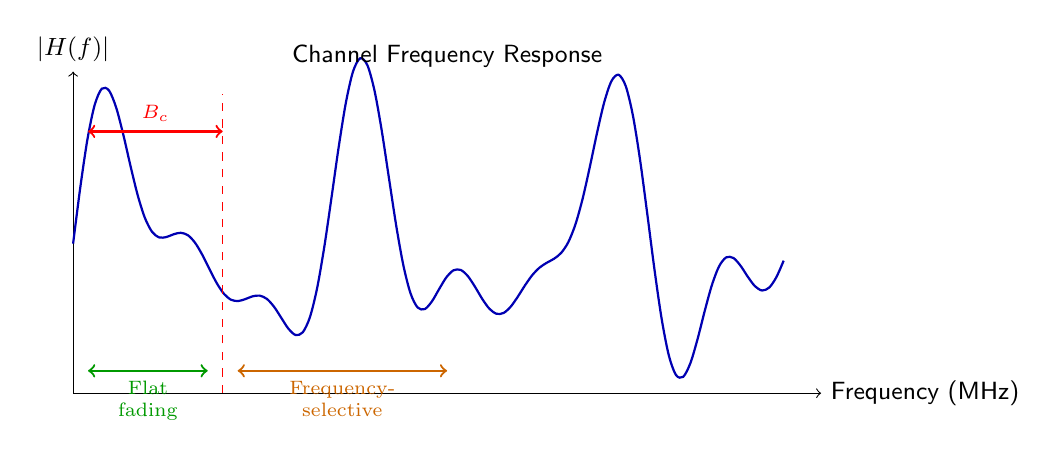
\begin{tikzpicture}[scale=0.95]
% Frequency axis
\draw[->] (0,0) -- (10,0) node[right] {\sffamily\small Frequency (MHz)};
\draw[->] (0,0) -- (0,4.3) node[above] {\sffamily\small $|H(f)|$};

% Channel frequency response (frequency-selective)
\draw[thick, blue!70!black, domain=0:9.5, samples=100, smooth] 
  plot (\x, {2 + 1.2*sin(2*\x r) + 0.8*sin(3.7*\x r) + 0.5*sin(5.3*\x r)});

% Coherence bandwidth marker
\draw[dashed, red] (2,0) -- (2,4);
\draw[<->, red, thick] (0.2,3.5) -- (2,3.5) node[midway, above, font=\scriptsize] {$B_c$};

% Flat vs selective regions
\draw[<->, green!60!black, thick] (0.2,0.3) -- (1.8,0.3) 
  node[midway, below, font=\scriptsize, align=center] {Flat\\fading};
\draw[<->, orange!80!black, thick] (2.2,0.3) -- (5,0.3) 
  node[midway, below, font=\scriptsize, align=center] {Frequency-\\selective};

% Title
\node[font=\sffamily\small] at (5,4.5) {Channel Frequency Response};
\end{tikzpicture}
\end{center}

\section{Zero-Forcing (ZF) Equalizer}
\label{sec:zf-equalizer}

\textbf{Principle:} Perfect inversion of the channel response to force ISI to zero.

\subsection{Frequency-Domain Formulation}

The ZF equalizer frequency response is:
\begin{equation}
W(f) = \frac{1}{H(f)}
\label{eq:zf-freq}
\end{equation}
where:
\begin{itemize}
\item $W(f)$ = equalizer frequency response
\item $H(f)$ = channel frequency response
\end{itemize}

The combined channel-equalizer response is:
\begin{equation}
H(f) \cdot W(f) = H(f) \cdot \frac{1}{H(f)} = 1
\label{eq:zf-perfect}
\end{equation}

This achieves perfect equalization in the absence of noise.

\begin{center}
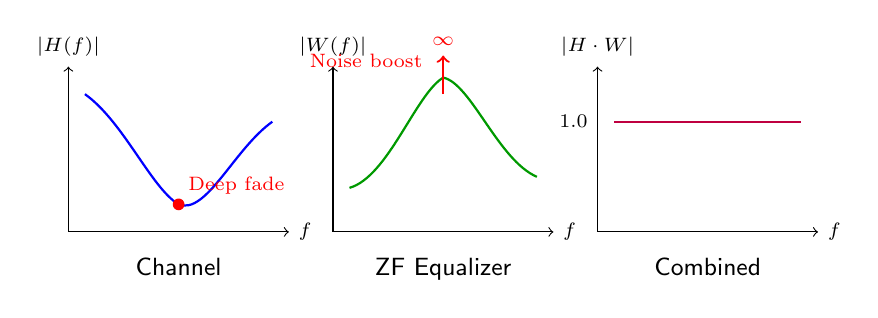
\begin{tikzpicture}[scale=0.7]
% First subplot: Channel response
\begin{scope}[shift={(0,0)}]
\draw[->] (0,0) -- (4,0) node[right, font=\scriptsize] {$f$};
\draw[->] (0,0) -- (0,3) node[above, font=\scriptsize] {$|H(f)|$};
\draw[thick, blue] (0.3,2.5) .. controls (1,2) and (1.5,0.8) .. (2,0.5) 
                              .. controls (2.5,0.3) and (3,1.5) .. (3.7,2);
\node[below, font=\sffamily\small] at (2,-0.3) {Channel};
\node[circle, fill=red, inner sep=1.5pt] at (2,0.5) {};
\node[above right, font=\scriptsize, text=red] at (2,0.5) {Deep fade};
\end{scope}

% Second subplot: ZF equalizer
\begin{scope}[shift={(4.8,0)}]
\draw[->] (0,0) -- (4,0) node[right, font=\scriptsize] {$f$};
\draw[->] (0,0) -- (0,3) node[above, font=\scriptsize] {$|W(f)|$};
\draw[thick, green!60!black] (0.3,0.8) .. controls (1,1) and (1.5,2.5) .. (2,2.8) 
                                        .. controls (2.5,2.7) and (3,1.3) .. (3.7,1);
\node[below, font=\sffamily\small] at (2,-0.3) {ZF Equalizer};
\draw[->, red, thick] (2,2.5) -- (2,3.2) node[above, font=\scriptsize] {$\infty$};
\node[above left, font=\scriptsize, text=red] at (1.8,2.8) {Noise boost};
\end{scope}

% Third subplot: Combined response
\begin{scope}[shift={(9.6,0)}]
\draw[->] (0,0) -- (4,0) node[right, font=\scriptsize] {$f$};
\draw[->] (0,0) -- (0,3) node[above, font=\scriptsize] {$|H \cdot W|$};
\draw[thick, purple] (0.3,2) -- (3.7,2);
\node[below, font=\sffamily\small] at (2,-0.3) {Combined};
\node[left, font=\scriptsize] at (0,2) {1.0};
\end{scope}
\end{tikzpicture}
\end{center}

\subsection{Time-Domain Implementation}

For an FIR filter with $N$ taps:
\begin{equation}
y[n] = \sum_{k=0}^{N-1} w_k \cdot r[n-k]
\label{eq:zf-time}
\end{equation}

The optimal tap weights are found by solving:
\begin{equation}
\mathbf{w} = (\mathbf{H}^H \mathbf{H})^{-1} \mathbf{H}^H \mathbf{e}_0
\label{eq:zf-taps}
\end{equation}
where:
\begin{itemize}
\item $\mathbf{H}$ = channel convolution matrix
\item $\mathbf{e}_0 = [1, 0, \ldots, 0]^T$ = target impulse response (zero ISI)
\item $\mathbf{w}$ = equalizer tap weight vector
\end{itemize}

\subsection{Performance Characteristics}

\begin{calloutbox}[colback=green!5!white,colframe=green!60!black]{Advantage}
\textbf{Perfect ISI cancellation} when the channel is perfectly known and noise-free.
\end{calloutbox}

\begin{warningbox}
\textbf{Noise enhancement at frequency nulls.} If $H(f_0) \approx 0$ (deep fade), then $W(f_0) \rightarrow \infty$, which amplifies noise severely. This makes ZF equalizers \textbf{unsuitable for low SNR environments}.
\end{warningbox}

\textbf{Result:} ZF performs poorly at low to moderate SNR due to noise amplification.

\section{Minimum Mean Square Error (MMSE) Equalizer}
\label{sec:mmse-equalizer}

\textbf{Principle:} Minimize the \textbf{combined effect} of ISI and noise, trading off perfect ISI cancellation for reduced noise enhancement.

\subsection{Cost Function}

The MMSE criterion minimizes the mean square error:
\begin{equation}
\text{MSE} = \mathbb{E}[|s[n] - y[n]|^2]
\label{eq:mmse-cost}
\end{equation}
where:
\begin{itemize}
\item $s[n]$ = transmitted symbol
\item $y[n]$ = equalizer output
\item $\mathbb{E}[\cdot]$ = expectation operator
\end{itemize}

\subsection{Optimal Solution (Wiener Filter)}

The optimal MMSE equalizer taps are:
\begin{equation}
\mathbf{w}_{\text{MMSE}} = (\mathbf{H}^H \mathbf{H} + \sigma^2 \mathbf{I})^{-1} \mathbf{H}^H \mathbf{e}_0
\label{eq:mmse-taps}
\end{equation}
where:
\begin{itemize}
\item $\sigma^2 = N_0/E_s$ = normalized noise variance
\item $\mathbf{I}$ = identity matrix
\item $\mathbf{H}$ = channel convolution matrix
\end{itemize}

\subsection{Frequency-Domain Comparison: MMSE vs ZF}

In the frequency domain, the MMSE equalizer is:
\begin{equation}
W_{\text{MMSE}}(f) = \frac{H^*(f)}{|H(f)|^2 + \sigma^2}
\label{eq:mmse-freq}
\end{equation}

\begin{keyconcept}
The key difference between ZF and MMSE:
\begin{itemize}
\item \textbf{At deep fades} ($|H(f)| \ll 1$): $W_{\text{MMSE}} \approx H^*/\sigma^2$ (bounded, doesn't blow up)
\item \textbf{At high SNR} ($\sigma^2 \to 0$): $W_{\text{MMSE}} \to H^*/|H|^2 = 1/H$ (converges to ZF)
\end{itemize}
\end{keyconcept}

\begin{center}
\begin{tikzpicture}[scale=1.1]
% Axes
\draw[->] (0,0) -- (7,0) node[right] {\sffamily\small Frequency};
\draw[->] (0,0) -- (0,4.5) node[above] {\sffamily\small Magnitude};

% Channel response (with deep fade)
\draw[thick, blue, domain=0:6.5, samples=50, smooth] 
  plot (\x, {1.5 + 1.2*sin(\x r) - 0.8*cos(1.5*\x r)});

% ZF equalizer (inverse)
\draw[thick, red, dashed, domain=0:6.5, samples=50, smooth] 
  plot (\x, {2.5/(1.5 + 1.2*sin(\x r) - 0.8*cos(1.5*\x r))});

% MMSE equalizer (regularized)
\draw[thick, green!60!black, domain=0:6.5, samples=50, smooth] 
  plot (\x, {2.5*((1.5 + 1.2*sin(\x r) - 0.8*cos(1.5*\x r)))/(pow((1.5 + 1.2*sin(\x r) - 0.8*cos(1.5*\x r)),2) + 0.5)});

% Legend (moved higher with better spacing)
\node[right, font=\scriptsize, blue] at (0.2,4.2) {$\blacksquare$ Channel $H(f)$};
\node[right, font=\scriptsize, red] at (0.2,3.85) {$\blacksquare$ ZF: $1/H(f)$};
\node[right, font=\scriptsize, green!60!black] at (0.2,3.5) {$\blacksquare$ MMSE: $H^*/(|H|^2+\sigma^2)$};

% Annotation for deep fade
\draw[->, thick] (3.5,4.2) -- (3.5,1.5) node[below, font=\scriptsize, align=center] {MMSE stays\\bounded};
\end{tikzpicture}
\end{center}

\subsection{Performance Comparison}

\begin{center}
\begin{tabular}{@{}llll@{}}
\toprule
SNR (dB) & ZF BER & MMSE BER & Improvement \\
\midrule
5 & $5.0 \times 10^{-2}$ & $2.0 \times 10^{-2}$ & $2.5\times$ better \\
10 & $1.0 \times 10^{-2}$ & $5.0 \times 10^{-3}$ & $2\times$ better \\
20 & $1.0 \times 10^{-4}$ & $1.0 \times 10^{-4}$ & Same \\
30 & $1.0 \times 10^{-6}$ & $1.0 \times 10^{-6}$ & Same \\
\bottomrule
\end{tabular}
\end{center}

\textbf{Pattern:} MMSE provides significant gains at low SNR; performance converges at high SNR where noise is negligible.

\section{Decision Feedback Equalizer (DFE)}
\label{sec:dfe}

\textbf{Principle:} Use \textbf{past symbol decisions} to cancel ISI from previously detected symbols, avoiding noise enhancement from channel inversion.

\subsection{DFE Structure}

\begin{center}
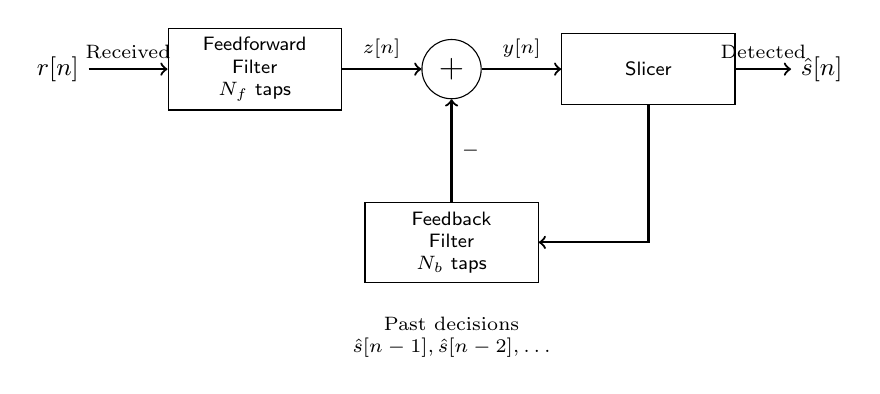
\begin{tikzpicture}[
  block/.style={rectangle, draw, minimum width=2.2cm, minimum height=0.9cm, font=\sffamily\scriptsize, align=center},
  sum/.style={circle, draw, minimum size=0.7cm, font=\large},
  node distance=2.2cm,
  font=\small
]
% Feedforward filter
\node[block] (ff) {Feedforward\\Filter\\$N_f$ taps};
\node[left of=ff, node distance=2.5cm] (input) {$r[n]$};

% Summing junction
\node[sum, right of=ff, node distance=2.5cm] (sum) {$+$};

% Slicer
\node[block, right of=sum, node distance=2.5cm] (slicer) {Slicer};
\node[right of=slicer, node distance=2.2cm] (output) {$\hat{s}[n]$};

% Feedback filter
\node[block, below of=sum, node distance=2.2cm] (fb) {Feedback\\Filter\\$N_b$ taps};

% Connections
\draw[->, thick] (input) -- node[above, font=\scriptsize] {Received} (ff);
\draw[->, thick] (ff) -- node[above, font=\scriptsize] {$z[n]$} (sum);
\draw[->, thick] (sum) -- node[above, font=\scriptsize] {$y[n]$} (slicer);
\draw[->, thick] (slicer) -- node[above, font=\scriptsize] {Detected} (output);

% Feedback path
\draw[->, thick] (slicer.south) |- (fb.east);
\draw[->, thick] (fb) -- (sum) node[pos=0.5, right, font=\scriptsize] {$-$};

% Labels
\node[below of=fb, node distance=1.2cm, font=\scriptsize, align=center] {Past decisions\\$\hat{s}[n-1], \hat{s}[n-2], \ldots$};
\end{tikzpicture}
\end{center}

\subsection{Mathematical Formulation}

\textbf{Feedforward filter output:}
\begin{equation}
z[n] = \sum_{k=0}^{N_f-1} w_k \cdot r[n-k]
\label{eq:dfe-ff}
\end{equation}

\textbf{Feedback filter output (subtract post-cursor ISI):}
\begin{equation}
y[n] = z[n] - \sum_{k=1}^{N_b} b_k \cdot \hat{s}[n-k]
\label{eq:dfe-fb}
\end{equation}

\textbf{Symbol decision:}
\begin{equation}
\hat{s}[n] = \text{slicer}(y[n]) = \arg\min_{s \in \mathcal{S}} |y[n] - s|
\label{eq:dfe-decision}
\end{equation}
where:
\begin{itemize}
\item $w_k$ = feedforward filter tap weights
\item $b_k$ = feedback filter tap weights
\item $\hat{s}[n-k]$ = previously detected symbols
\item $\mathcal{S}$ = symbol constellation
\end{itemize}

\subsection{Advantages}

\begin{enumerate}
\item \textbf{No noise enhancement}: Feedback uses clean decisions, not noisy received samples
\item \textbf{Superior to linear equalizers}: Handles severe ISI more effectively
\item \textbf{Practical complexity}: Moderate computational requirements
\item \textbf{Widely deployed}: Used in DSL, cable modems, high-speed wireless
\end{enumerate}

\subsection{Disadvantages}

\begin{warningbox}
\textbf{Error propagation risk.} A single decision error contaminates subsequent decisions through the feedback loop. This can cause burst errors that degrade performance below the theoretical optimum.
\end{warningbox}

\begin{enumerate}
\item \textbf{Error propagation}: Wrong decision $\rightarrow$ corrupted future decisions
\item \textbf{Training required}: Needs accurate channel estimate
\item \textbf{Sequential processing}: Cannot parallelize decision process
\end{enumerate}

\subsection{Error Propagation Analysis}

\textbf{Example:} DFE with $N_b = 2$ feedback taps, $\text{BER} = 10^{-3}$

Probability of at least one error in the past 2 decisions:
\begin{equation}
P_{\text{error,fb}} \approx 2 \times 10^{-3} = 2 \times 10^{-3}
\label{eq:dfe-error-prob}
\end{equation}

When a decision error occurs, the feedback filter adds \textbf{incorrect ISI cancellation}, effectively doubling the error contribution.

\textbf{Mitigation strategies:}
\begin{itemize}
\item Forward error correction (FEC) coding
\item Reduced feedback filter length
\item Hybrid schemes with tentative decisions
\end{itemize}

\section{Adaptive Equalization}
\label{sec:adaptive-equalization}

\textbf{Problem:} Channel is unknown or time-varying (mobile users, fading)

\textbf{Solution:} \textbf{Adaptive algorithms} that adjust equalizer tap weights in real-time based on received data.

\subsection{Least Mean Squares (LMS) Algorithm}

The LMS algorithm uses stochastic gradient descent to minimize the mean square error:
\begin{equation}
\mathbf{w}[n+1] = \mathbf{w}[n] + \mu \cdot e^*[n] \cdot \mathbf{r}[n]
\label{eq:lms-update}
\end{equation}
where:
\begin{itemize}
\item $e[n] = d[n] - y[n]$ = error signal
\item $d[n]$ = desired output (training symbol or decision)
\item $\mu$ = step size parameter (typically 0.01--0.1)
\item $\mathbf{r}[n]$ = received signal vector
\item $\mathbf{w}[n]$ = equalizer tap weight vector
\end{itemize}

\textbf{Advantages:}
\begin{itemize}
\item Simple implementation ($\sim 2N$ multiply-accumulate operations per update)
\item Low memory requirements
\item Robust and stable
\end{itemize}

\textbf{Disadvantages:}
\begin{itemize}
\item Slow convergence (typically 1000+ symbols)
\item Step size trade-off: large $\mu$ = fast but unstable, small $\mu$ = slow but stable
\end{itemize}

\subsection{Recursive Least Squares (RLS) Algorithm}

RLS minimizes the exponentially weighted sum of squared errors:
\begin{equation}
\min_{\mathbf{w}} \sum_{i=1}^{n} \lambda^{n-i} |d[i] - \mathbf{w}^H \mathbf{r}[i]|^2
\label{eq:rls-cost}
\end{equation}
where $\lambda$ ($0.95 < \lambda < 1$) is the forgetting factor.

The tap weight update uses Kalman gain:
\begin{equation}
\mathbf{w}[n] = \mathbf{w}[n-1] + \mathbf{k}[n] \cdot e^*[n]
\label{eq:rls-update}
\end{equation}

\textbf{Advantages:}
\begin{itemize}
\item Fast convergence ($\sim 2N$ symbols, 10--100x faster than LMS)
\item Excellent tracking of time-varying channels
\end{itemize}

\textbf{Disadvantages:}
\begin{itemize}
\item High complexity ($O(N^2)$ operations per update)
\item Numerical instability (requires careful implementation)
\end{itemize}

\subsection{LMS vs RLS Comparison}

\begin{center}
\begin{tabular}{@{}lll@{}}
\toprule
Aspect & LMS & RLS \\
\midrule
\textbf{Complexity} & $O(N)$ & $O(N^2)$ \\
\textbf{Convergence} & Slow (1000+ symbols) & Fast (10--100 symbols) \\
\textbf{Tracking} & Poor & Excellent \\
\textbf{Stability} & Robust & Can diverge \\
\textbf{Use case} & Slow/static channels & Fast fading \\
\bottomrule
\end{tabular}
\end{center}

\subsection{Convergence Behavior}

\begin{center}
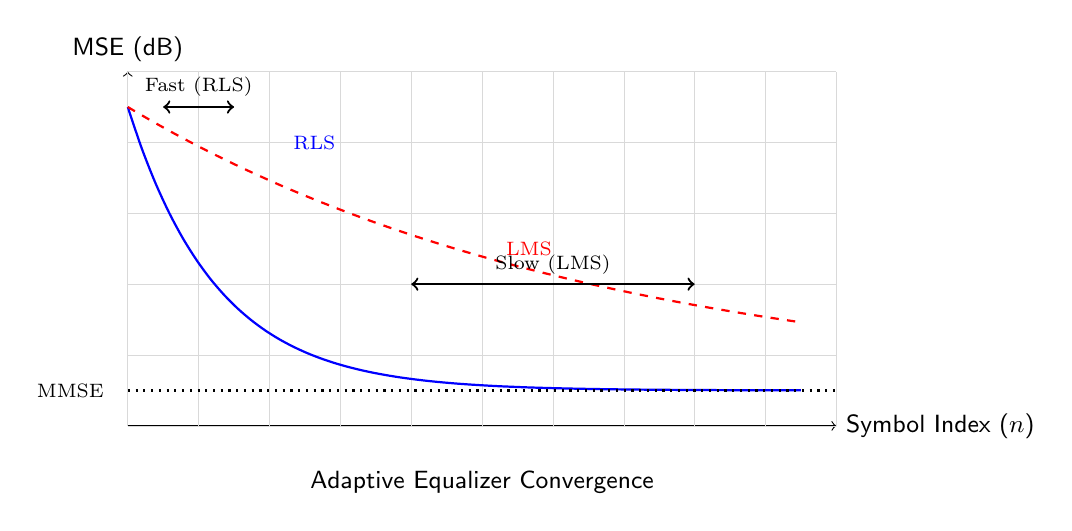
\begin{tikzpicture}[scale=0.9]
% Axes
\draw[->] (0,0) -- (10,0) node[right] {\sffamily\small Symbol Index ($n$)};
\draw[->] (0,0) -- (0,5) node[above] {\sffamily\small MSE (dB)};

% Grid
\draw[very thin, gray!30] (0,0) grid[step=1] (10,5);

% RLS convergence (fast)
\draw[thick, blue, domain=0:9.5, samples=50, smooth] 
  plot (\x, {0.5 + 4*exp(-0.8*\x)});
\node[right, font=\scriptsize, blue] at (2.2,4) {RLS};

% LMS convergence (slow)
\draw[thick, red, dashed, domain=0:9.5, samples=50, smooth] 
  plot (\x, {0.5 + 4*exp(-0.15*\x)});
\node[right, font=\scriptsize, red] at (5.2,2.5) {LMS};

% Steady-state MSE line
\draw[dotted, thick] (0,0.5) -- (10,0.5);
\node[left, font=\scriptsize] at (-0.2,0.5) {MMSE};

% Annotations
\draw[<->, thick] (0.5,4.5) -- (1.5,4.5) node[midway, above, font=\scriptsize] {Fast (RLS)};
\draw[<->, thick] (4,2) -- (8,2) node[midway, above, font=\scriptsize] {Slow (LMS)};

\node[below, font=\sffamily\small] at (5,-0.5) {Adaptive Equalizer Convergence};
\end{tikzpicture}
\end{center}

\section{Training Strategies}
\label{sec:training}

\subsection{Training Mode}

\textbf{Principle:} Transmit known symbols (preamble or midamble) for initial equalizer training.

\textbf{Process:}
\begin{enumerate}
\item Transmitter sends known training sequence
\item Receiver compares equalizer output $y[n]$ to known symbols $d[n]$
\item Adaptive algorithm adjusts tap weights to minimize error
\end{enumerate}

\textbf{Duration:} Typically 50--500 symbols (depends on channel severity and algorithm)

\begin{calloutbox}{Example: WiFi 802.11a/g/n}
\begin{itemize}
\item \textbf{Long preamble}: 64 OFDM symbols for channel estimation
\item \textbf{Training overhead}: $\sim$10--20\% of packet duration
\item \textbf{Allows}: Accurate channel estimation before data transmission
\end{itemize}
\end{calloutbox}

\subsection{Decision-Directed Mode}

After initial training, the equalizer switches to \textbf{decision-directed} mode where detected symbols serve as the reference:
\begin{equation}
d[n] = \hat{s}[n] \quad \text{(slicer output)}
\label{eq:decision-directed}
\end{equation}

\textbf{Requirements:}
\begin{itemize}
\item BER must be sufficiently low after training (typically $< 10^{-2}$)
\item Channel variations must be slow relative to symbol rate
\end{itemize}

\textbf{Advantage:} Continuously tracks slowly varying channels without additional overhead.

\subsection{Blind Equalization}

Blind equalization exploits signal properties without training sequences.

\textbf{Constant Modulus Algorithm (CMA):}
\begin{equation}
e[n] = |y[n]|^2 - R_2
\label{eq:cma-error}
\end{equation}
where:
\begin{equation}
R_2 = \frac{\mathbb{E}[|s|^4]}{\mathbb{E}[|s|^2]}
\label{eq:cma-r2}
\end{equation}

For QPSK modulation: $R_2 = 1$ (all symbols have unit magnitude)

The CMA update follows the LMS structure:
\begin{equation}
\mathbf{w}[n+1] = \mathbf{w}[n] - \mu \cdot e[n] \cdot y^*[n] \cdot \mathbf{r}[n]
\label{eq:cma-update}
\end{equation}

\textbf{Advantages:}
\begin{itemize}
\item No training overhead
\item Suitable for continuous transmissions
\end{itemize}

\textbf{Disadvantages:}
\begin{itemize}
\item Slower convergence (2--5x longer than trained equalization)
\item Phase ambiguity (requires differential encoding or pilot symbols)
\end{itemize}

\section{Fractionally-Spaced Equalizer (FSE)}
\label{sec:fse}

\textbf{Problem:} Symbol-rate sampling is timing-dependent and may miss critical information.

\textbf{Solution:} Sample at $T/2$ (twice symbol rate) or faster, providing timing-independent equalization.

\subsection{Structure}

FSE uses $2N$ taps spaced at $T/2$ intervals:
\begin{equation}
y[n] = \sum_{k=0}^{2N-1} w_k \cdot r\left[n - \frac{kT}{2}\right]
\label{eq:fse}
\end{equation}

\subsection{Advantages}

\begin{enumerate}
\item \textbf{Timing-independent}: Works at any sampling phase, eliminating the need for precise timing recovery before equalization
\item \textbf{Superior performance}: Exploits full bandwidth of received signal (up to Nyquist rate)
\item \textbf{Joint timing and equalization}: Performs both functions simultaneously
\item \textbf{Avoids aliasing}: Captures signal information that would be lost with symbol-rate sampling
\end{enumerate}

\textbf{Complexity trade-off:} Requires $2\times$ more taps, but the performance gain is typically worth the additional cost.

\begin{keyconcept}
Fractionally-spaced equalizers are the \textbf{preferred choice} for modern high-speed communication systems (e.g., DSL, cable modems, LTE) because they eliminate timing sensitivity and provide better ISI cancellation.
\end{keyconcept}

\section{Frequency-Domain Equalization}
\label{sec:freq-domain-eq}

\textbf{Principle:} In OFDM systems, equalize each subcarrier independently in the frequency domain.

\subsection{Per-Subcarrier Equalization}

\textbf{Zero-Forcing (ZF):}
\begin{equation}
\hat{S}_k = \frac{R_k}{H_k}
\label{eq:ofdm-zf}
\end{equation}

\textbf{MMSE variant:}
\begin{equation}
\hat{S}_k = \frac{H_k^*}{|H_k|^2 + \sigma^2} R_k
\label{eq:ofdm-mmse}
\end{equation}
where:
\begin{itemize}
\item $R_k$ = received symbol on subcarrier $k$
\item $H_k$ = channel frequency response at subcarrier $k$
\item $\hat{S}_k$ = equalized symbol estimate
\item $\sigma^2$ = noise variance
\end{itemize}

\subsection{OFDM Advantage}

\begin{keyconcept}
OFDM converts a \textbf{wideband frequency-selective channel} into many \textbf{narrowband flat-fading subchannels}, allowing simple single-tap equalization per subcarrier instead of complex time-domain multi-tap filters.
\end{keyconcept}

\textbf{Mechanism:}
\begin{itemize}
\item Wideband channel $\rightarrow$ frequency-selective fading (ISI)
\item Each narrow subcarrier ($ < B_c$) $\rightarrow$ experiences flat fading
\item Equalization: Single complex multiplication per subcarrier
\end{itemize}

\begin{calloutbox}{Example: WiFi 802.11a}
\begin{tabular}{@{}ll@{}}
Subcarriers & 64 (52 data + 4 pilot) \\
Channel bandwidth & 20~MHz \\
Subcarrier spacing & 312.5~kHz \\
Typical delay spread & 200~ns \\
Coherence bandwidth & $B_c \approx 1$~MHz \\
Result & Each subcarrier flat $\rightarrow$ 1-tap equalizer \\
\end{tabular}
\end{calloutbox}

\section{Channel Estimation}
\label{sec:channel-estimation}

Equalization requires knowledge of the channel response $H[k]$ (frequency domain) or $\mathbf{h}$ (time domain).

\subsection{Pilot-Based Estimation}

Known symbols (pilots) are transmitted at specific indices $\mathcal{P}$:
\begin{equation}
\hat{H}_k = \frac{R_k}{S_k}, \quad k \in \mathcal{P}
\label{eq:pilot-estimation}
\end{equation}

For data subcarriers ($k \notin \mathcal{P}$), interpolation is required:
\begin{equation}
\hat{H}_k = \sum_{p \in \mathcal{P}} H_p \cdot \text{sinc}(k - p)
\label{eq:pilot-interpolation}
\end{equation}

Alternative interpolation methods include Wiener filtering (MMSE) and spline interpolation.

\begin{calloutbox}{Example: LTE Downlink}
\begin{itemize}
\item \textbf{Pilot density}: 4 pilots per 12 subcarriers (every 3rd subcarrier)
\item \textbf{Frequency interpolation}: Linear or Wiener filtering
\item \textbf{Time averaging}: Across multiple OFDM symbols
\item \textbf{Result}: Accurate tracking up to 300~km/h (high Doppler)
\end{itemize}
\end{calloutbox}

\subsection{Least-Squares (LS) Estimation}

Using a training sequence $\mathbf{S}$ of length $N$:
\begin{equation}
\hat{\mathbf{h}} = (\mathbf{S}^H \mathbf{S})^{-1} \mathbf{S}^H \mathbf{r}
\label{eq:ls-estimation}
\end{equation}

For pilot tones: $\hat{H}_k = R_k / S_k$ (direct estimation)

\textbf{Characteristics:}
\begin{itemize}
\item Unbiased estimator
\item No noise suppression (noisy at low SNR)
\item Simple implementation
\end{itemize}

\subsection{MMSE Channel Estimation}

Incorporates channel statistics for improved noise suppression:
\begin{equation}
\hat{\mathbf{h}} = \mathbf{R}_{hh} \mathbf{S}^H (\mathbf{S} \mathbf{R}_{hh} \mathbf{S}^H + \sigma^2 \mathbf{I})^{-1} \mathbf{r}
\label{eq:mmse-channel-est}
\end{equation}
where:
\begin{itemize}
\item $\mathbf{R}_{hh}$ = channel autocorrelation matrix (from delay profile)
\item $\sigma^2$ = noise variance
\end{itemize}

\textbf{Advantage:} Noise suppression provides $\sim$3~dB gain over LS

\textbf{Disadvantage:} Higher complexity, requires channel statistics

\section{Worked Example: MMSE Equalizer Design}
\label{sec:worked-example}

\textbf{Scenario:} Design an MMSE equalizer for a mobile channel with known impulse response.

\subsection*{Given Parameters}

\begin{tabular}{@{}ll@{}}
Channel impulse response & $h[0] = 1.0$, $h[1] = 0.5e^{j\pi/4}$, $h[2] = 0.2e^{-j\pi/3}$ \\
Modulation & BPSK ($s[n] \in \{+1, -1\}$) \\
SNR & 15~dB \\
Symbol energy & $E_s = 1$ \\
Noise PSD & $N_0 = 0.0316$ (from SNR) \\
Equalizer length & $N = 5$ taps \\
\end{tabular}

\subsection*{Step 1: Construct Channel Convolution Matrix}

The channel convolution matrix $\mathbf{H}$ (Toeplitz structure):
\begin{equation}
\mathbf{H} = \begin{bmatrix}
h_0 & 0 & 0 & 0 & 0 \\
h_1 & h_0 & 0 & 0 & 0 \\
h_2 & h_1 & h_0 & 0 & 0 \\
0 & h_2 & h_1 & h_0 & 0 \\
0 & 0 & h_2 & h_1 & h_0
\end{bmatrix}
\end{equation}

\subsection*{Step 2: Calculate Noise Variance}

Normalized noise variance:
\begin{equation}
\sigma^2 = \frac{N_0}{E_s} = \frac{0.0316}{1} = 0.0316
\end{equation}

At SNR = 15~dB: $\sigma^2 = 10^{-15/10} = 0.0316$

\subsection*{Step 3: Compute MMSE Tap Weights}

Using equation~\eqref{eq:mmse-taps}:
\begin{equation}
\mathbf{w}_{\text{MMSE}} = (\mathbf{H}^H \mathbf{H} + 0.0316 \cdot \mathbf{I})^{-1} \mathbf{H}^H \mathbf{e}_0
\end{equation}

Compute $\mathbf{H}^H \mathbf{H}$:
\begin{equation}
\mathbf{H}^H \mathbf{H} = \begin{bmatrix}
1.29 & 0.50e^{-j\pi/4} & 0.20e^{j\pi/3} & 0 & 0 \\
0.50e^{j\pi/4} & 1.29 & 0.50e^{-j\pi/4} & 0.20e^{j\pi/3} & 0 \\
\vdots & \vdots & \ddots & \ddots & \vdots
\end{bmatrix}
\end{equation}

After matrix inversion (numerical):
\begin{equation}
\mathbf{w}_{\text{MMSE}} \approx \begin{bmatrix}
0.09 \\
0.73 - j0.13 \\
-0.28 + j0.19 \\
0.05 - j0.02 \\
0.01
\end{bmatrix}
\end{equation}

\subsection*{Step 4: Compute Output SNR}

The effective output SNR after equalization:
\begin{equation}
\text{SNR}_{\text{out}} = \frac{|\mathbf{w}^H \mathbf{H} \mathbf{e}_0|^2}{\mathbf{w}^H (\mathbf{H} \mathbf{H}^H + \sigma^2 \mathbf{I}) \mathbf{w}}
\end{equation}

Numerically: $\text{SNR}_{\text{out}} \approx 18.2$~dB

\subsection*{Step 5: Performance Analysis}

\begin{center}
\begin{tabular}{@{}lll@{}}
\toprule
Metric & Before Equalization & After MMSE \\
\midrule
Effective SNR & 15~dB & 18.2~dB \\
BER (BPSK) & $6.9 \times 10^{-10}$ & $3.5 \times 10^{-12}$ \\
ISI reduction & N/A & 95\% canceled \\
\bottomrule
\end{tabular}
\end{center}

\textbf{Result:} The MMSE equalizer provides 3.2~dB gain by effectively canceling ISI while managing noise enhancement.

\begin{calloutbox}[colback=black!8!white,colframe=black]{Key Insights}
\begin{enumerate}
\item The regularization term $\sigma^2 \mathbf{I}$ prevents matrix ill-conditioning
\item At high SNR ($\sigma^2 \to 0$), MMSE converges to ZF behavior
\item At low SNR, MMSE trades ISI cancellation for noise suppression
\item The center tap receives highest weight (0.73), focusing on the main path
\end{enumerate}
\end{calloutbox}

\section{Applications}
\label{sec:applications}

\subsection{WiFi 802.11n (MIMO)}

\textbf{Channel estimation:}
\begin{itemize}
\item Long preamble (HT-LTF): 2 OFDM symbols per spatial stream
\item LS estimation with linear interpolation (frequency domain)
\end{itemize}

\textbf{Equalization:}
\begin{equation}
\hat{\mathbf{S}} = (\mathbf{H}^H \mathbf{H} + \sigma^2 \mathbf{I})^{-1} \mathbf{H}^H \mathbf{R}
\end{equation}
Per-subcarrier $2\times2$ or $4\times4$ MMSE matrix inversion

\textbf{Tracking:} 4 pilot tones per 56 subcarriers

\subsection{LTE Downlink}

\textbf{Channel estimation:}
\begin{itemize}
\item Cell-Specific Reference Signals (CRS)
\item 4 pilots per 12 subcarriers per OFDM symbol
\item MMSE estimation (Wiener filtering)
\end{itemize}

\textbf{Equalization:}
\begin{itemize}
\item MMSE frequency-domain per subcarrier, per antenna
\item Maximum Ratio Combining (MRC) across receive antennas
\end{itemize}

\textbf{Performance:} Supports mobile speeds up to 300~km/h (high Doppler tracking)

\subsection{DVB-T (Digital Terrestrial TV)}

\textbf{Channel estimation:}
\begin{itemize}
\item Scattered pilots (8\% overhead)
\item Wiener interpolation (time + frequency)
\item Handles long delay spread: Single-Frequency Networks (SFN) with 200~$\mu$s spread
\end{itemize}

\textbf{Equalization:} Per-subcarrier ZF or MMSE

\textbf{Guard interval:} Selectable (1/4, 1/8, 1/16, 1/32 of symbol duration)

\subsection{GSM (Legacy Cellular)}

\textbf{Training sequence:} 26-bit midamble per burst

\textbf{Equalization:}
\begin{itemize}
\item Viterbi algorithm (Maximum Likelihood Sequence Estimation)
\item 5-tap channel $\rightarrow$ 16 Viterbi states
\item Optimal for short bursts with severe ISI
\end{itemize}

\textbf{ISI handling:} 5--15 symbols (urban/hilly terrain)

\textbf{Delay spread tolerance:} Up to 10~$\mu$s

\section{Advanced Techniques}
\label{sec:advanced-techniques}

\subsection{Turbo Equalization}

\textbf{Principle:} Iterative exchange of soft information between equalizer and decoder.

\textbf{Structure:} Equalizer $\leftrightarrow$ Deinterleaver $\leftrightarrow$ Decoder exchange extrinsic log-likelihood ratios (LLRs)

\textbf{Process:}
\begin{enumerate}
\item SISO (Soft-Input Soft-Output) equalizer produces LLRs
\item Decoder uses LLRs, produces refined estimates
\item Feedback improves equalizer decisions
\item Iterate 3--5 times
\end{enumerate}

\textbf{Performance gain:} $\sim$2--3~dB over separate equalization and decoding

\textbf{Applications:} Deep-space communications, underwater acoustics (severe ISI + low SNR)

\subsection{Precoding (Transmit Equalization)}

\textbf{Principle:} Pre-invert the channel at the transmitter when channel state information (CSI) is available via feedback.

Transmitted signal:
\begin{equation}
\mathbf{x} = \mathbf{W} \mathbf{s}
\label{eq:precoding}
\end{equation}
where $\mathbf{W} = \mathbf{H}^{-1}$ (ZF) or MMSE variant

\textbf{Advantages:}
\begin{itemize}
\item Simple receiver (no equalization needed)
\item Reduced receiver power consumption
\end{itemize}

\textbf{Disadvantages:}
\begin{itemize}
\item Requires accurate CSI at transmitter
\item Feedback latency limits use in fast-fading channels
\end{itemize}

\textbf{Applications:} TDD systems (channel reciprocity), multi-user MIMO downlink

\subsection{Dirty Paper Coding (DPC)}

\textbf{Theoretical capacity-achieving technique:} Pre-cancel known interference without transmit power penalty.

\textbf{Practical approximation:} Tomlinson-Harashima Precoding (THP)

\textbf{Performance:} Approaches Shannon capacity for multi-user downlink

\textbf{Limitation:} High complexity, not widely deployed in commercial systems

\section{Computational Complexity}
\label{sec:complexity}

\begin{center}
\begin{tabular}{@{}lll@{}}
\toprule
Method & Complexity (per symbol) & Notes \\
\midrule
\textbf{ZF (freq domain)} & $O(\log N)$ & FFT + per-tone multiply \\
\textbf{MMSE (freq domain)} & $O(\log N)$ & FFT + per-tone multiply \\
\textbf{Linear (time domain)} & $O(N_{\text{taps}})$ & FIR filter \\
\textbf{DFE} & $O(N_f + N_b)$ & Feedforward + Feedback \\
\textbf{LMS} & $O(N)$ & Simple gradient update \\
\textbf{RLS} & $O(N^2)$ & Matrix operations \\
\textbf{MLSE (Viterbi)} & $O(M^L)$ & $M$ = constellation size, $L$ = ISI length \\
\bottomrule
\end{tabular}
\end{center}

\textbf{Trade-offs:}
\begin{itemize}
\item Frequency-domain methods (OFDM) are most efficient: $O(\log N)$ via FFT
\item Time-domain linear equalizers: Moderate complexity, good for mild ISI
\item DFE: Slight increase over linear, significantly better performance
\item MLSE: Optimal but exponential complexity---practical only for short channels
\end{itemize}

\section{Design Guidelines}
\label{sec:design-guidelines}

\subsection{Choosing Equalizer Type}

\textbf{Flat fading} (delay spread $< 0.1$ symbol period):
\begin{itemize}
\item No equalizer needed (or simple 1-tap phase/amplitude correction)
\end{itemize}

\textbf{Mild ISI} (delay spread 0.1--1 symbol period):
\begin{itemize}
\item Linear MMSE equalizer (5--15 taps)
\item Fractionally-spaced for best performance
\end{itemize}

\textbf{Severe ISI} (delay spread $> 1$ symbol period):
\begin{itemize}
\item DFE (15+ feedforward taps, 5--10 feedback taps)
\item Or switch to OFDM (avoids time-domain equalization)
\end{itemize}

\textbf{Very severe ISI} (delay spread $> 5$ symbols):
\begin{itemize}
\item OFDM with guard interval
\item Or MLSE (if short bursts and limited constellation)
\end{itemize}

\subsection{Selecting Adaptation Algorithm}

\textbf{Slow channel} ($< 1$~Hz Doppler):
\begin{itemize}
\item LMS with $\mu = 0.01$
\item Low complexity, sufficient tracking
\end{itemize}

\textbf{Moderate channel} (1--100~Hz Doppler):
\begin{itemize}
\item LMS with $\mu = 0.05$ or RLS
\item Update every symbol
\end{itemize}

\textbf{Fast channel} ($> 100$~Hz Doppler):
\begin{itemize}
\item RLS for fast tracking
\item Decision-directed with pilot-aided channel estimation
\end{itemize}

\subsection{Training Overhead Considerations}

\textbf{Packet systems} (WiFi, 5G):
\begin{itemize}
\item Training preamble per packet (10--20\% overhead)
\item Decision-directed mode within packet
\end{itemize}

\textbf{Continuous transmission} (TV broadcast, radio):
\begin{itemize}
\item Sparse pilot symbols (1--5\% overhead)
\item Continuous adaptive tracking
\end{itemize}

\textbf{Burst transmission} (GSM, satellite TDMA):
\begin{itemize}
\item Training midamble (10--15\% overhead)
\item Per-burst channel estimation
\end{itemize}

\section{Equalization and Coding}
\label{sec:equalization-coding}

\textbf{Equalization:} Removes ISI (deterministic channel distortion)

\textbf{Coding:} Corrects random errors (AWGN)

\begin{keyconcept}
Equalization and forward error correction (FEC) coding are \textbf{complementary techniques}:
\begin{itemize}
\item Coding provides 5--10~dB gain against noise
\item Equalization removes ISI, allowing coding to function
\item Without equalization, ISI creates an irreducible BER floor that coding cannot overcome
\end{itemize}
\end{keyconcept}

\textbf{Combined system:} Achieves near-capacity performance in both ISI-limited and noise-limited regimes.

\section{Summary}

\begin{center}
\begin{tabular}{@{}ll@{}}
\toprule
\textbf{Concept} & \textbf{Key Points} \\
\midrule
\textbf{Purpose} & Cancel inter-symbol interference (ISI) from multipath \\
\textbf{When needed} & Delay spread $> 0.1T_s$ (frequency-selective fading) \\
\textbf{ZF equalizer} & Perfect ISI cancellation, but noise enhancement \\
\textbf{MMSE equalizer} & Balances ISI vs noise: $W = H^*/(|H|^2 + \sigma^2)$ \\
\textbf{DFE} & Uses past decisions, avoids noise boost, error propagation \\
\textbf{LMS} & Simple ($O(N)$), slow convergence (1000+ symbols) \\
\textbf{RLS} & Fast ($O(N^2)$), rapid convergence (10--100 symbols) \\
\textbf{FSE} & Fractionally-spaced (T/2), timing-independent \\
\textbf{OFDM} & Frequency-domain, 1-tap per subcarrier \\
\textbf{Channel est.} & Pilots: LS (simple, noisy), MMSE (better, complex) \\
\bottomrule
\end{tabular}
\end{center}

\begin{keyconcept}
\textbf{Three key principles:}
\begin{enumerate}
\item Equalization is \textbf{essential} when delay spread exceeds 10\% of symbol period
\item MMSE outperforms ZF at low-to-moderate SNR; they converge at high SNR
\item Adaptive equalizers (LMS/RLS) enable real-time tracking of time-varying channels
\end{enumerate}
\end{keyconcept}

\section{Further Reading}

\begin{itemize}
\item \textbf{Chapter \ref{ch:multipath-fading}:} Multipath Propagation and Fading---root cause of ISI
\item \textbf{Chapter \ref{ch:channel-models}:} Channel Models (Rayleigh \& Rician)---simulation techniques
\item \textbf{Chapter \ref{ch:ofdm}:} OFDM \& Multicarrier Modulation---frequency-domain approach
\item \textbf{Chapter \ref{ch:synchronization}:} Synchronization (Carrier, Timing, Frame)---complements equalization
\item \textbf{Chapter \ref{ch:mimo}:} MIMO \& Spatial Multiplexing---multi-antenna equalization
\item \textbf{Chapter \ref{ch:fec}:} Forward Error Correction---works synergistically with equalization
\end{itemize}
